\documentclass{beamer}
%
% Choose how your presentation looks.
%
% For more themes, color themes and font themes, see:
% http://deic.uab.es/~iblanes/beamer_gallery/index_by_theme.html
%
\mode<presentation>
{
  \usetheme{default}      % or try Darmstadt, Madrid, Warsaw, ...
  \usecolortheme{default} % or try albatross, beaver, crane, ...
  \usefonttheme{default}  % or try serif, structurebold, ...
  \setbeamertemplate{navigation symbols}{}
  \setbeamertemplate{caption}[numbered]
} 

\usepackage[english]{babel}
\usepackage[utf8x]{inputenc}
\usepackage{hyperref}

%%%%%%%%%%%%%%%%%%%%%%%%%%%%%%%%%%%%%%%%%%%%%
% Slide 1
\title[Sandhi]{Sandhi}
\author{Manoj Gudi}
\institute{Ex-R.A. FOSSEE | CTO | FocusAnalytics}
\date{3rd December 2014}

\begin{document}
\begin{frame}
  \titlepage
\end{frame}

% Uncomment these lines for an automatically generated outline.
%\begin{frame}{Outline}
%  \tableofcontents
%\end{frame}

\section{Introduction}

%%%%%%%%%%%%%%%%%%%%%%%%%%%%%%%%%%%%%%%%%%%%%%
% Slide 2
\begin{frame}{Pre-Sandhi}

\begin{itemize}
  \item LabVIEW: A proprietary visual programming software by NI
  \item Vendor lockdown 
  \item Buy NI DAC cards .. Buy LabVIEW  = \textbf{ \textit{Expensive Maxx}}
  \item Little care for support on Free Operating Systems: GNU/Linux.
  \item Initial target: Virtual Labs, IIT Bombay.
\end{itemize}
\vskip 1cm
\end{frame}

%%%%%%%%%%%%%%%%%%%%%%%%%%%%%%%%%%%%%%%%%%%%%%%
% Slide 3
\section{Virtual labs meme}
\vskip 1cm
\begin{frame}{}
\subsection{section}
\begin{figure} [ht!]
	\centering
	
\includegraphics[width=70mm]{meme1.jpg}
\end{figure}
\end{frame}

%%%%%%%%%%%%%%%%%%%%%%%%%%%%%%%%%%%%%%%%%%%%%%%%
% Slide4
\section{Sandhi basic features}
\begin{frame}{Objectives}
\begin{figure} [ht!]
	\centering
	
\includegraphics[width=60mm]{meme2.jpg}
\end{figure}

\begin{itemize}
  \item Free and Open source
  \item Easy to use | Clean interface | Drag \& Drop 
  \item Should run on GNU/Linux smoothly
  \item Able to carry out control system experiments
  \item Framework should support \textbf{feedbacks}
\end{itemize}
\vskip 1cm
\end{frame}
%%%%%%%%%%%%%%%%%%%%%%%%%%%%%%%%%%%%%%%%%%%%%

% Slide 5
\section{Sandhi Architecture image}
\begin{frame}{Architecture}

\begin{figure} [ht!]
	\centering
	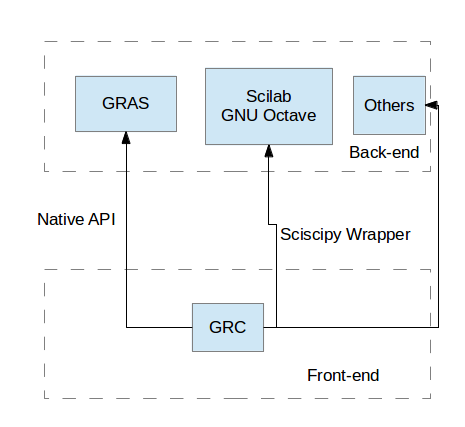
\includegraphics[width=80mm]{image.png}
\end{figure}
\vskip 1cm
\end{frame}
%%%%%%%%%%%%%%%%%%%%%%%%%%%%%%%%%%%%%%%%%%%%%

% Slide 6
\section{Sandhi Basic Features}
\begin{frame}{Features}

\begin{itemize}
  \item Light-weight \textasciitilde 20mb without depdendencies
  \item Good Hardware driver support
  \item Language support for Development: Scilab, GNU/Octave, Python, C++
  \item Developed for Control system application
  \item But can be easily extended for
  \begin{itemize}
  	\item Image Processing*
	\item Neural Networks*
	\item And any other areas which can be represented as data-flowgraph
  \end{itemize}
\end{itemize}
\vskip 1cm
\end{frame}


%%%%%%%%%%%%%%%%%%%%%%%%%%%%%%%%%%%%%%%%%%%%%

% Slide 7
\begin{frame}{Sandhi \textless3 Scilab}

\begin{itemize}
  \item Sciscipy wrapper - Sylvestre Ledru and Vincent Guffens
  \item Sample code
  \begin{itemize}\item \textit{from scilab import Scilab 
                \\  sci = Scilab()
                \\  x = sci.rand(20, 20)
                \\  y = x*x.transpose()
                \\  y\_inv = sci.inv(y)}
  \end{itemize}
  \item RIP: Linker Bug [2011-13]
  \item Fixed for Scilab 5.4+  YEAH!
  \item Use pure* functions of Scilab directly
  \item Provides way to evaluate code-string too.
\end{itemize}
\vskip 1cm
\end{frame}

%%%%%%%%%%%%%%%%%%%%%%%%%%%%%%%%%%%%%%%%%%%%%

% Slide 8
\section{Current Development I}
\begin{frame}{Current Approach:Functional Approach}

\begin{itemize}
  \item Referential Transparency (Pure and Impure Functions)
  \item Using GNU Radio's rudimentary type checker
  \item Function composition = \textit{complex becomes simple}
  \item Few impure functions are inherited from GNU Radio
  \item if \textit{(software == reliable)} then \textit{blame(hardware\_guys)}
\end{itemize}
\vskip 1cm
\end{frame}

%%%%%%%%%%%%%%%%%%%%%%%%%%%%%%%%%%%%%%%%%%%%
% Slide 9
\section{Current Development II}
\begin{frame}{Exciting features in pipeline}

\begin{itemize}
  \item HaPy Wrapper (David Fischer)integrated and tested (for Pure functions)
  \begin{itemize}
    \item Terse and elegant code
    \item Compiled and faster
    \item Immutable objects means easily \textit{parallelizable}
  \end{itemize}
  \item Shifting to cloud based architecture(using RPC)
  \begin{itemize}
    \item A client side containing smaller GRC, runtime environment
    \item Server side containing heaviy libraries
    \item Prototyped using RabbitMQ's RPC service(AQMP)
    \item Should work well for heavy simulations (if not realtime app)
  \end{itemize}
  \item Functional block generator
\end{itemize}
\vskip 1cm
\end{frame}

%%%%%%%%%%%%%%%%%%%%%%%%%%%%%%%%%%%%%%%%%%%%
% Slide 10
\begin{frame}{References/Links}

\begin{itemize}
  \item Source code \url{https://github.com/gnu-sandhi/sandhi.git}
  \item Documentation \url{https://github.com/gnu-sandhi/docs.git}
  \item Problems using it? Found a bug?
  \begin{itemize}
 	\item Are you sure its a bug and \textbf{not} \textit{a feature}?
	\item Raise an issue on our github
	\item Mailing List: \textit{gnu\_lc@googlegroups.com}
  \end{itemize}
\end{itemize}

\vskip 1cm

\end{frame}
%%%%%%%%%%%%%%%%%%%%%%%%%%%%%%%%%%%%%%%%%%%%%

\end{document}
